% ================================================================
% Section 3 — Data Collection & Methodology (RQ2 portion)
% Paste this block inside your \section{Data Collection \& Methodology}
% ================================================================

\subsection{RQ2: Measuring Sentiment Drift Across Epochs}
\label{subsec:rq2-method}

\subsubsection{Sentiment Scoring with VADER}

To measure how the emotional tone of AI coverage changes over time, we apply
VADER (Valence Aware Dictionary and sEntiment Reasoner)~\cite{hutto2014vader}
to each article. VADER is a lexicon-based model that assigns a
\textit{compound} score in $[-1,\,1]$, where scores above $+0.5$ are
\textit{strongly positive}, scores below $-0.5$ are \textit{strongly
negative}, and scores within $\pm 0.05$ are \textit{neutral}. We chose VADER
because it works well on short, journalistic text and requires no
labelled training data.

We score two text fields per article: (1)~the \textbf{abstract} (primary
signal) and (2)~the \textbf{headline} (secondary signal). The abstract
contains richer context than the headline and is therefore used as the main
signal for all statistical comparisons.

\subsubsection{Epoch Partitioning}

We divide the 2000--2025 timeline into three non-overlapping epochs that
reflect well-known turning points in AI development:

\begin{itemize}
  \item \textbf{Era~1 (2000--2011) --- Pre-deep-learning.} AI coverage
  during this period centred on expert systems, early robotics, and
  speculative futures.
  \item \textbf{Era~2 (2012--2018) --- Deep-learning expansion.} Triggered
  by AlexNet's breakthrough at ImageNet 2012, this era saw rapid progress in
  computer vision and natural language processing.
  \item \textbf{Era~3 (2019--2025) --- Generative-AI integration.} Defined
  by the rise of large language models (GPT-2 through GPT-4) and the public
  launch of ChatGPT in late 2022, which brought AI into mainstream public
  discourse.
\end{itemize}

The same three-epoch structure is used in RQ1, allowing direct comparison
between topic prevalence and sentiment trends.

\subsubsection{Statistical Testing}

Compound sentiment scores are not normally distributed, so we use the
two-sided \textbf{Mann-Whitney U test} rather than a t-test to compare
epoch pairs. We use $p < 0.05$ as the threshold for statistical significance.
Effect size is reported as the rank-biserial correlation $r$, defined as
$r = 1 - 2U / (n_1 n_2)$, where larger $|r|$ means a stronger practical
difference between epochs. We test all three pairwise comparisons
(Era~1 vs.\ Era~2, Era~2 vs.\ Era~3, and Era~1 vs.\ Era~3).

\subsubsection{Data Preparation}

The RQ2 corpus is the same as the one used in RQ1. We loaded the NYT article
metadata from a CSV file covering 2000--2025 and kept only articles that
matched at least one AI-related keyword (e.g.,
\textit{artificial intelligence}, \textit{machine learning},
\textit{ChatGPT}, \textit{large language model}). Non-news item types such
as obituaries, letters, and reviews were removed, as were articles from
unrelated sections (Sports, Arts, Travel, Real Estate). This yielded
\textbf{1,087 articles} across all three epochs. Before scoring, each
abstract and headline was passed through a phrase-standardisation step
(e.g., ``large language model'' $\to$ \texttt{large\_language\_model}) to
prevent VADER from splitting multi-word AI terms into unrelated
sub-tokens.


% ================================================================
% Section 4 — Empirical Results and Analysis (RQ2 portion)
% Paste this block inside your \section{Empirical Results and Analysis}
% ================================================================

\subsection{RQ2: Sentiment Drift and Polarization in AI Coverage}
\label{subsec:rq2-results}

\subsubsection{Descriptive Statistics}

Table~\ref{tab:rq2-desc} shows the abstract-sentiment statistics for each
epoch. Mean compound scores decreased monotonically: Era~1 ($\mu = 0.210$),
Era~2 ($\mu = 0.153$), Era~3 ($\mu = 0.140$). This steady drop suggests
that NYT coverage of AI gradually became less positive over 25 years.

The proportion of \textit{strongly negative} articles rose from 7.1\%
(Era~1) to 6.2\% (Era~2) and then to 8.8\% (Era~3). At the same time, the
share of \textit{neutral} articles fell sharply in Era~3 (22.1\%) compared
with Era~1 (27.4\%) and Era~2 (28.2\%). This means that recent generative-AI
coverage tends to take a clearer stance rather than staying neutral.

The inter-quartile range (IQR) was highest in Era~3 (0.567), which indicates
greater spread across the sentiment spectrum in the most recent epoch---a
sign of increasing polarisation visible in the violin plots
(Figure~\ref{fig:rq2-violin}).

\begin{table}[t]
  \caption{Descriptive statistics of abstract VADER compound scores per
    epoch. IQR = inter-quartile range; \% Strong Neg.\ = percentage of
    articles with compound score $< -0.5$.}
  \label{tab:rq2-desc}
  \small
  \begin{tabular}{lrrrrr}
    \toprule
    Epoch            & $n$   & Mean   & Std    & IQR    & \% Neg. \\
    \midrule
    Era~1 (2000--2011) & 467 & 0.210  & 0.451  & 0.586  & 7.1 \\
    Era~2 (2012--2018) & 355 & 0.153  & 0.390  & 0.465  & 6.2 \\
    Era~3 (2019--2025) & 262 & 0.140  & 0.427  & 0.567  & 8.8 \\
    \bottomrule
  \end{tabular}
\end{table}

\subsubsection{Significance Tests}

Table~\ref{tab:rq2-tests} reports the pairwise Mann-Whitney U test results
for abstract compound scores.

The only statistically significant result is the comparison between Era~1
and Era~3 ($U = 66{,}678.5$, $p = 0.042$, $r = -0.090$). This confirms that
there is a reliable, albeit small, shift in sentiment polarity over the full
25-year period. The Era~1 vs.\ Era~2 comparison approaches but does not
reach significance ($p = 0.064$), while the Era~2 vs.\ Era~3 comparison
shows virtually no difference ($p = 0.798$). Headline-level tests were all
non-significant across all pairs (all $p > 0.08$), which is expected given
that news headlines tend to be factual and emotionally flat.

\begin{table}[t]
  \caption{Pairwise Mann-Whitney U test results for abstract sentiment. An
    asterisk (*) marks results significant at $p < 0.05$. $r$ = rank-biserial
    correlation (effect size).}
  \label{tab:rq2-tests}
  \small
  \begin{tabular}{llccc}
    \toprule
    Epoch A              & Epoch B              & $U$          & $p$    & $r$    \\
    \midrule
    Era~1 (2000--2011)   & Era~2 (2012--2018)   & 89,075.5     & 0.064  & $-$0.075 \\
    Era~2 (2012--2018)   & Era~3 (2019--2025)   & 47,063.0     & 0.798  & $-$0.012 \\
    Era~1 (2000--2011)   & Era~3 (2019--2025)   & 66,678.5     & 0.042* & $-$0.090 \\
    \bottomrule
  \end{tabular}
\end{table}

\subsubsection{Temporal Trends}

Figure~\ref{fig:rq2-mean} plots the year-by-year mean abstract sentiment
from 2000 to 2024. Sentiment was relatively high and variable in the early
2000s (peaking around 2003--2004 at $\mu \approx 0.32$), then trended
downward. Two notable dips appear around 2011 ($\mu = 0.057$) and
2017 ($\mu = 0.025$), likely reflecting growing media attention to
algorithmic bias and automation-related job concerns. A brief spike in
2018 ($\mu = 0.284$) and again in 2022 ($\mu = 0.273$) precedes a sharp
drop in 2023 ($\mu = 0.137$) and 2024 ($\mu = 0.133$), coinciding with
widespread public debate over ChatGPT and generative AI safety.

Figure~\ref{fig:rq2-std} shows the annual standard deviation of compound
scores as a measure of dispersion (polarisation). Values remain moderate
throughout most of the timeline but climb in 2024 ($\sigma \approx 0.48$),
suggesting that while the average tone became slightly more negative, the
\textit{range} of opinions expressed in AI articles also widened in the
most recent years.

\subsubsection{Polarisation by Sentiment Category}

Figure~\ref{fig:rq2-proportions} breaks down each epoch into three
sentiment bands: strongly positive (compound $> 0.5$), neutral or mild, and
strongly negative (compound $< -0.5$). Era~3 stands out with the
smallest neutral share (22.1\%) and the largest strongly-negative share
(8.8\%), consistent with a media environment increasingly divided between
enthusiastic AI boosters and sharp critics.

\begin{figure}[t]
  \centering
  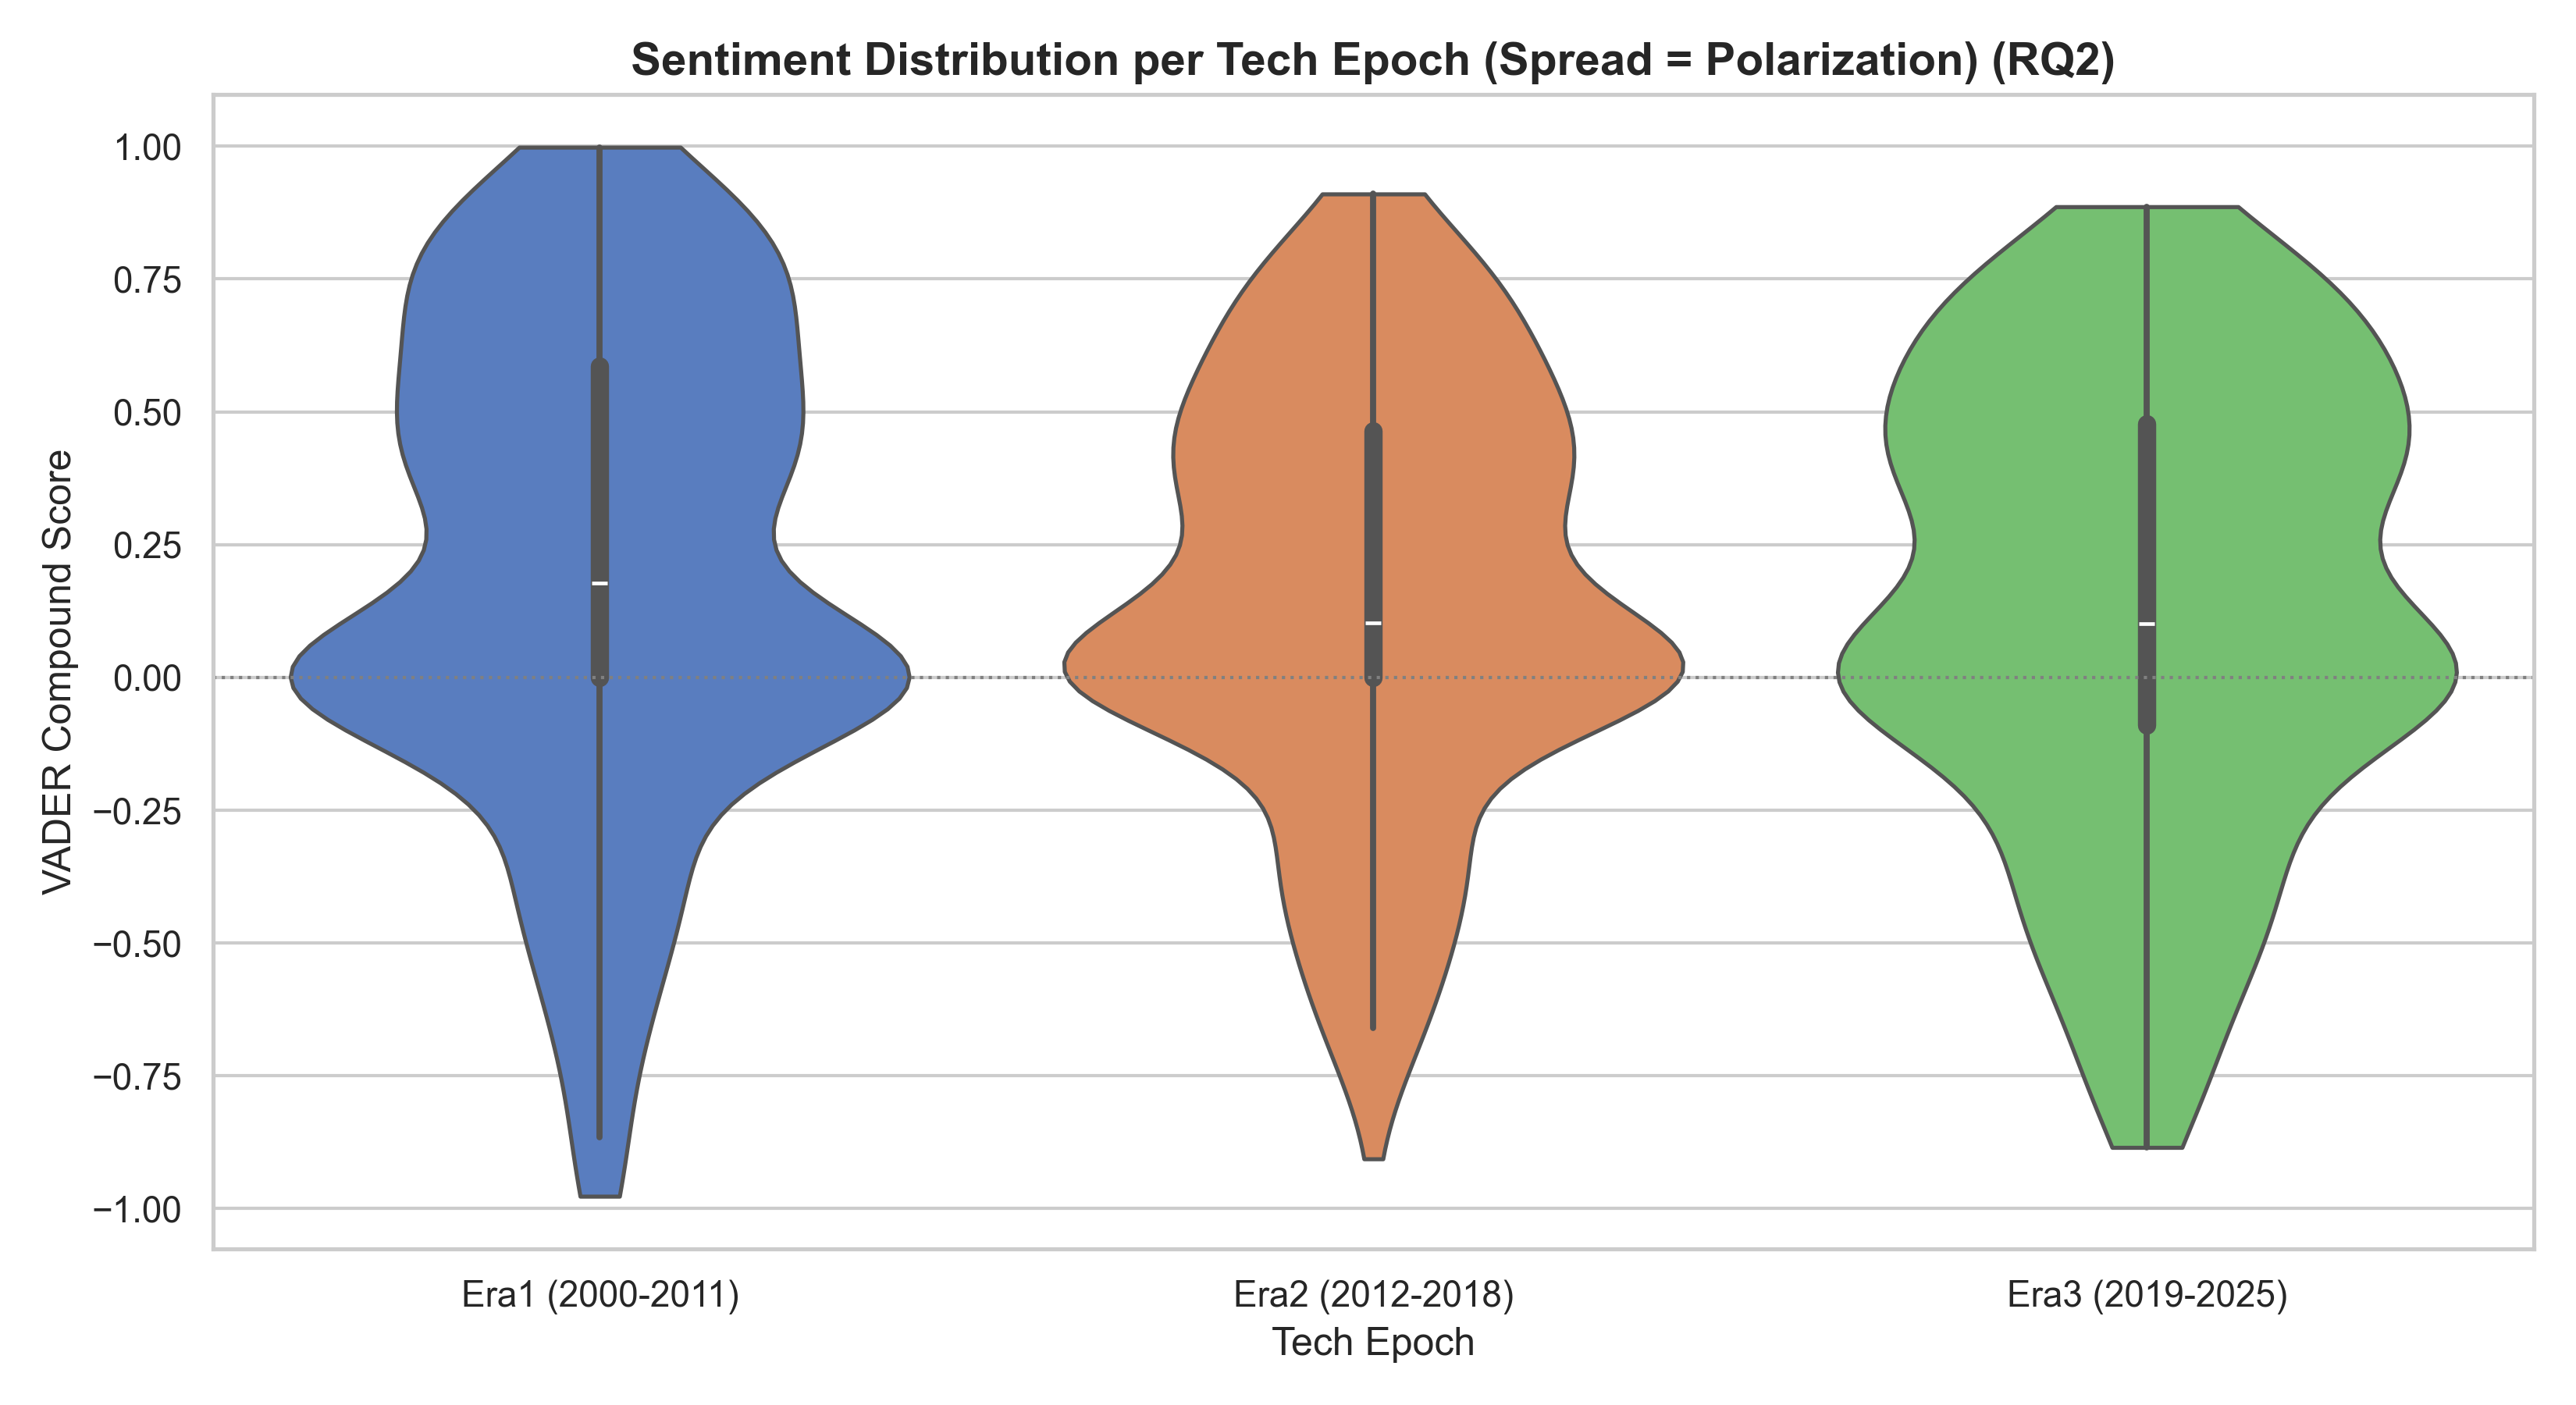
\includegraphics[width=\linewidth]{results/rq2_epoch_distributions.png}
  \caption{Violin plots of VADER compound scores per epoch. The wider shape
    of Era~3 relative to Era~2 reflects greater sentiment spread in the
    generative-AI period.}
  \label{fig:rq2-violin}
\end{figure}

\begin{figure}[t]
  \centering
  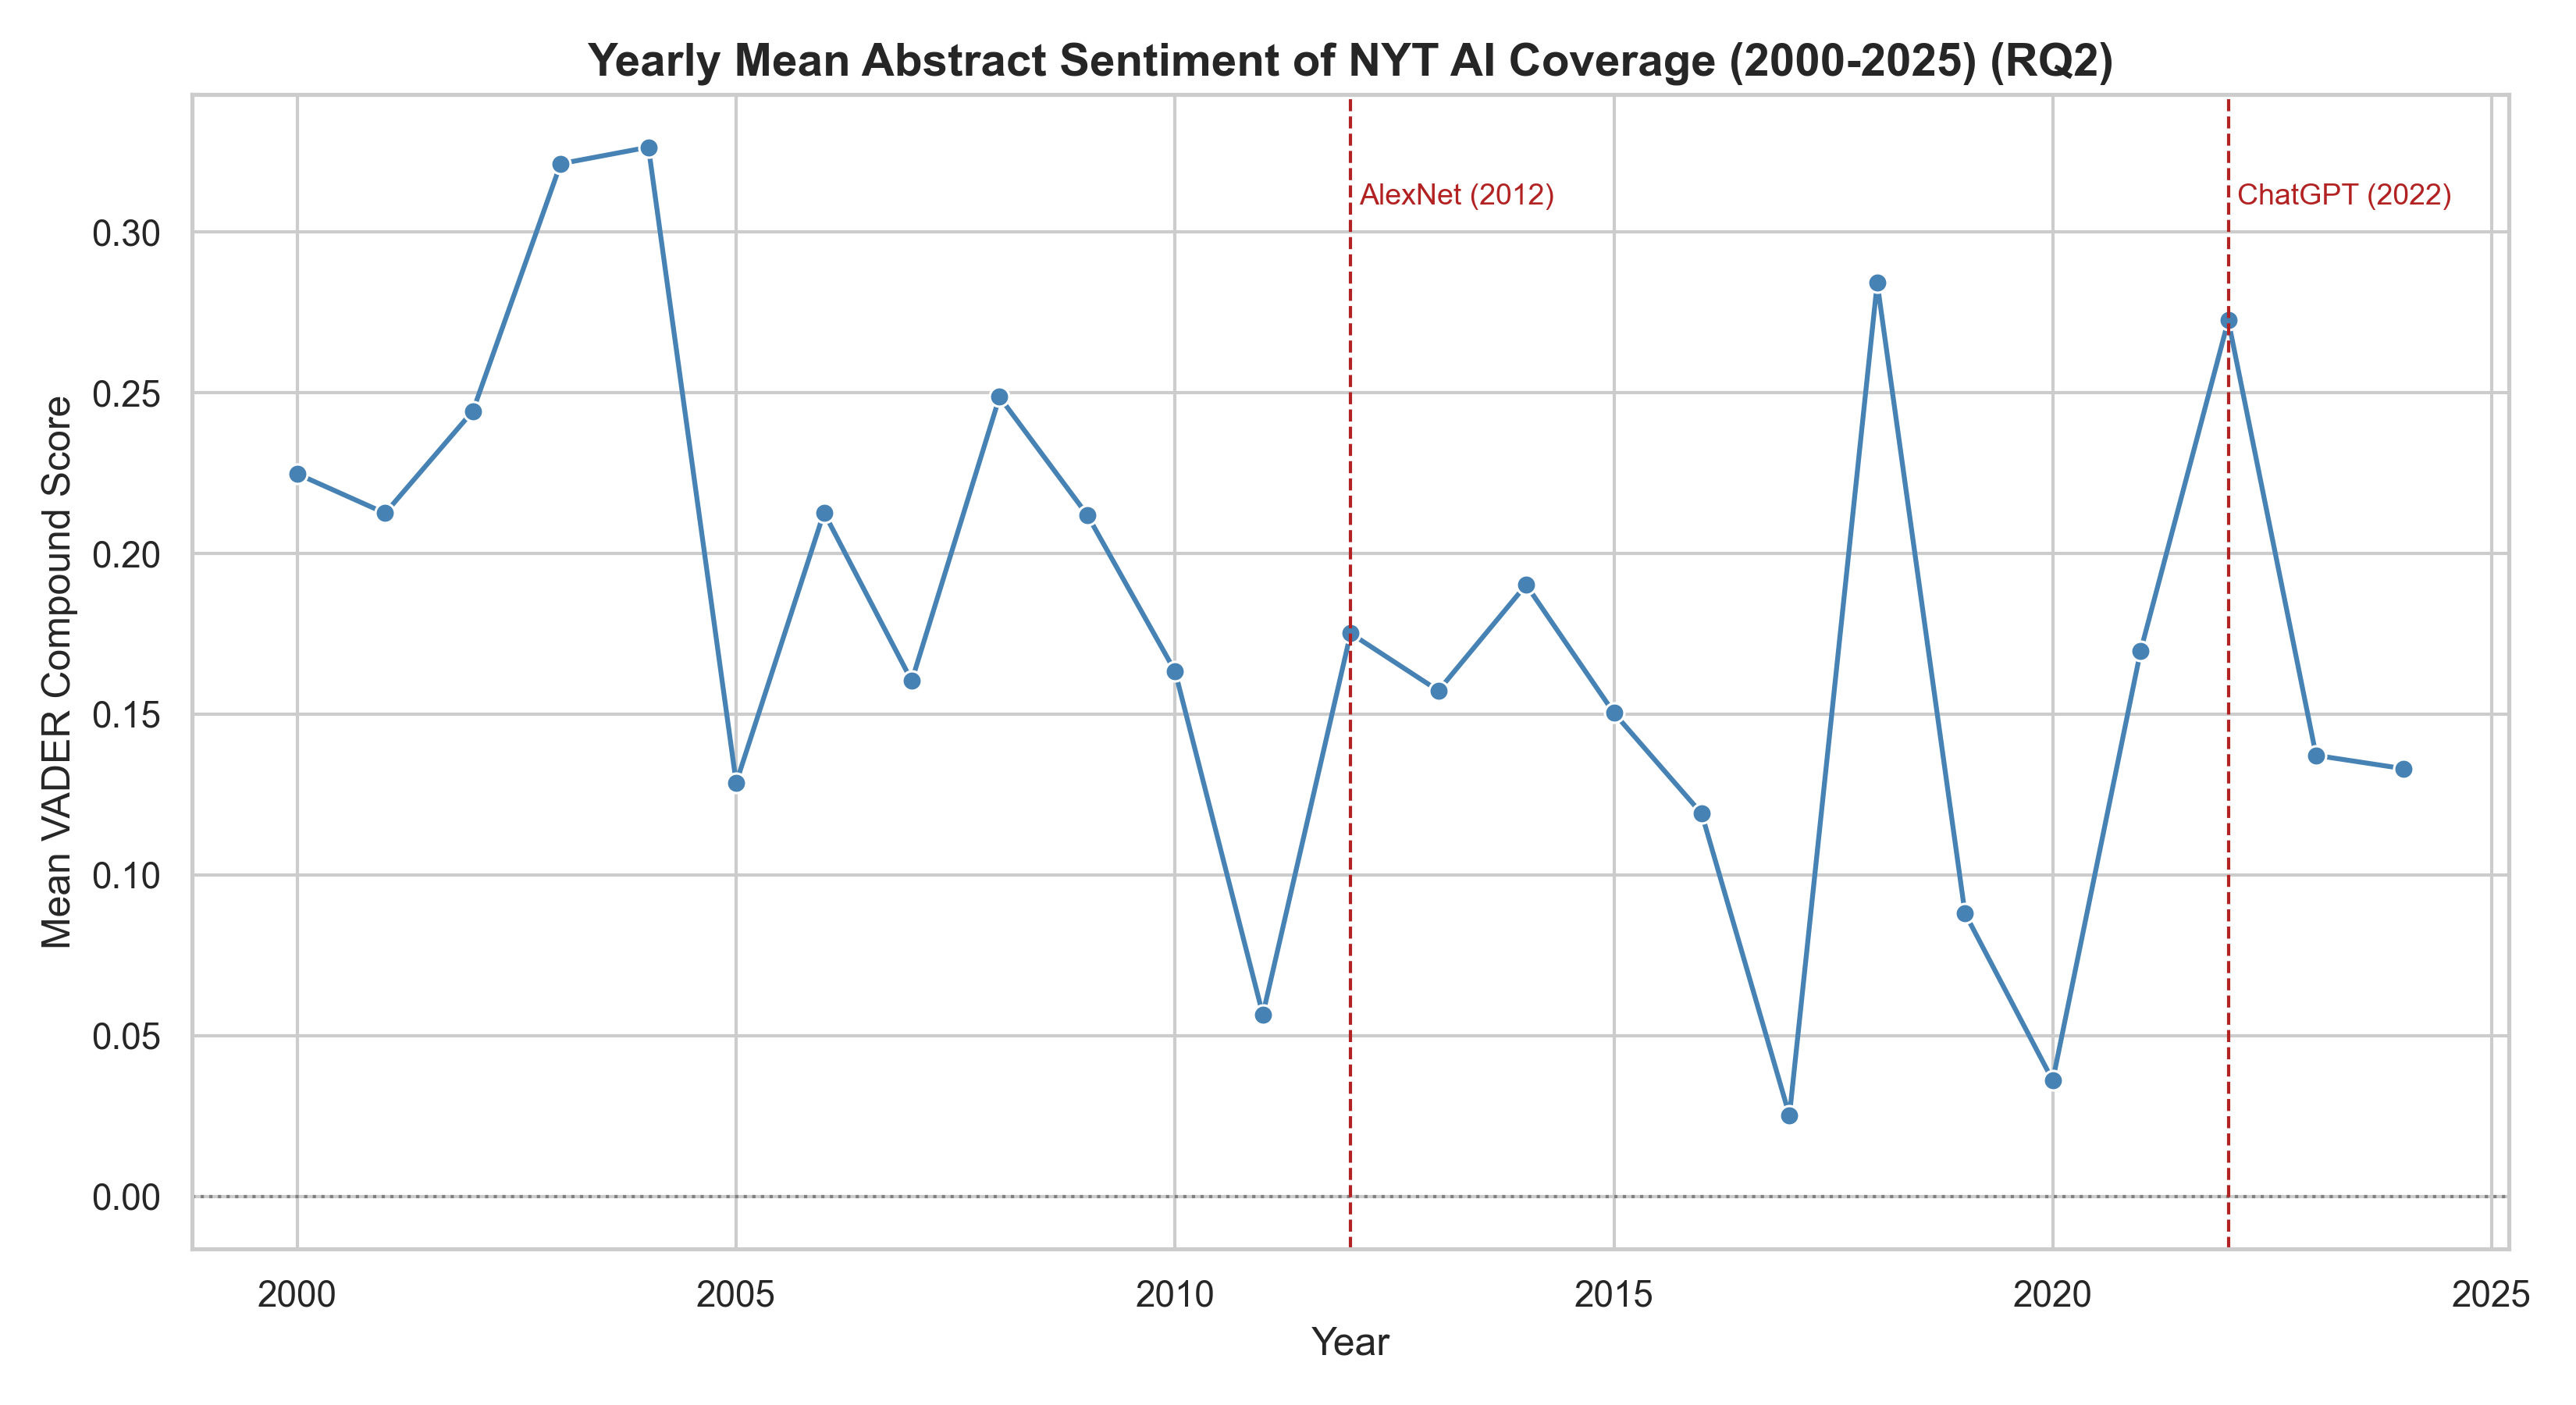
\includegraphics[width=\linewidth]{results/rq2_yearly_mean_sentiment.png}
  \caption{Year-by-year mean abstract sentiment in NYT AI-related articles
    (2000--2025). Vertical dashed lines mark the AlexNet milestone (2012)
    and the public release of ChatGPT (2022).}
  \label{fig:rq2-mean}
\end{figure}

\begin{figure}[t]
  \centering
  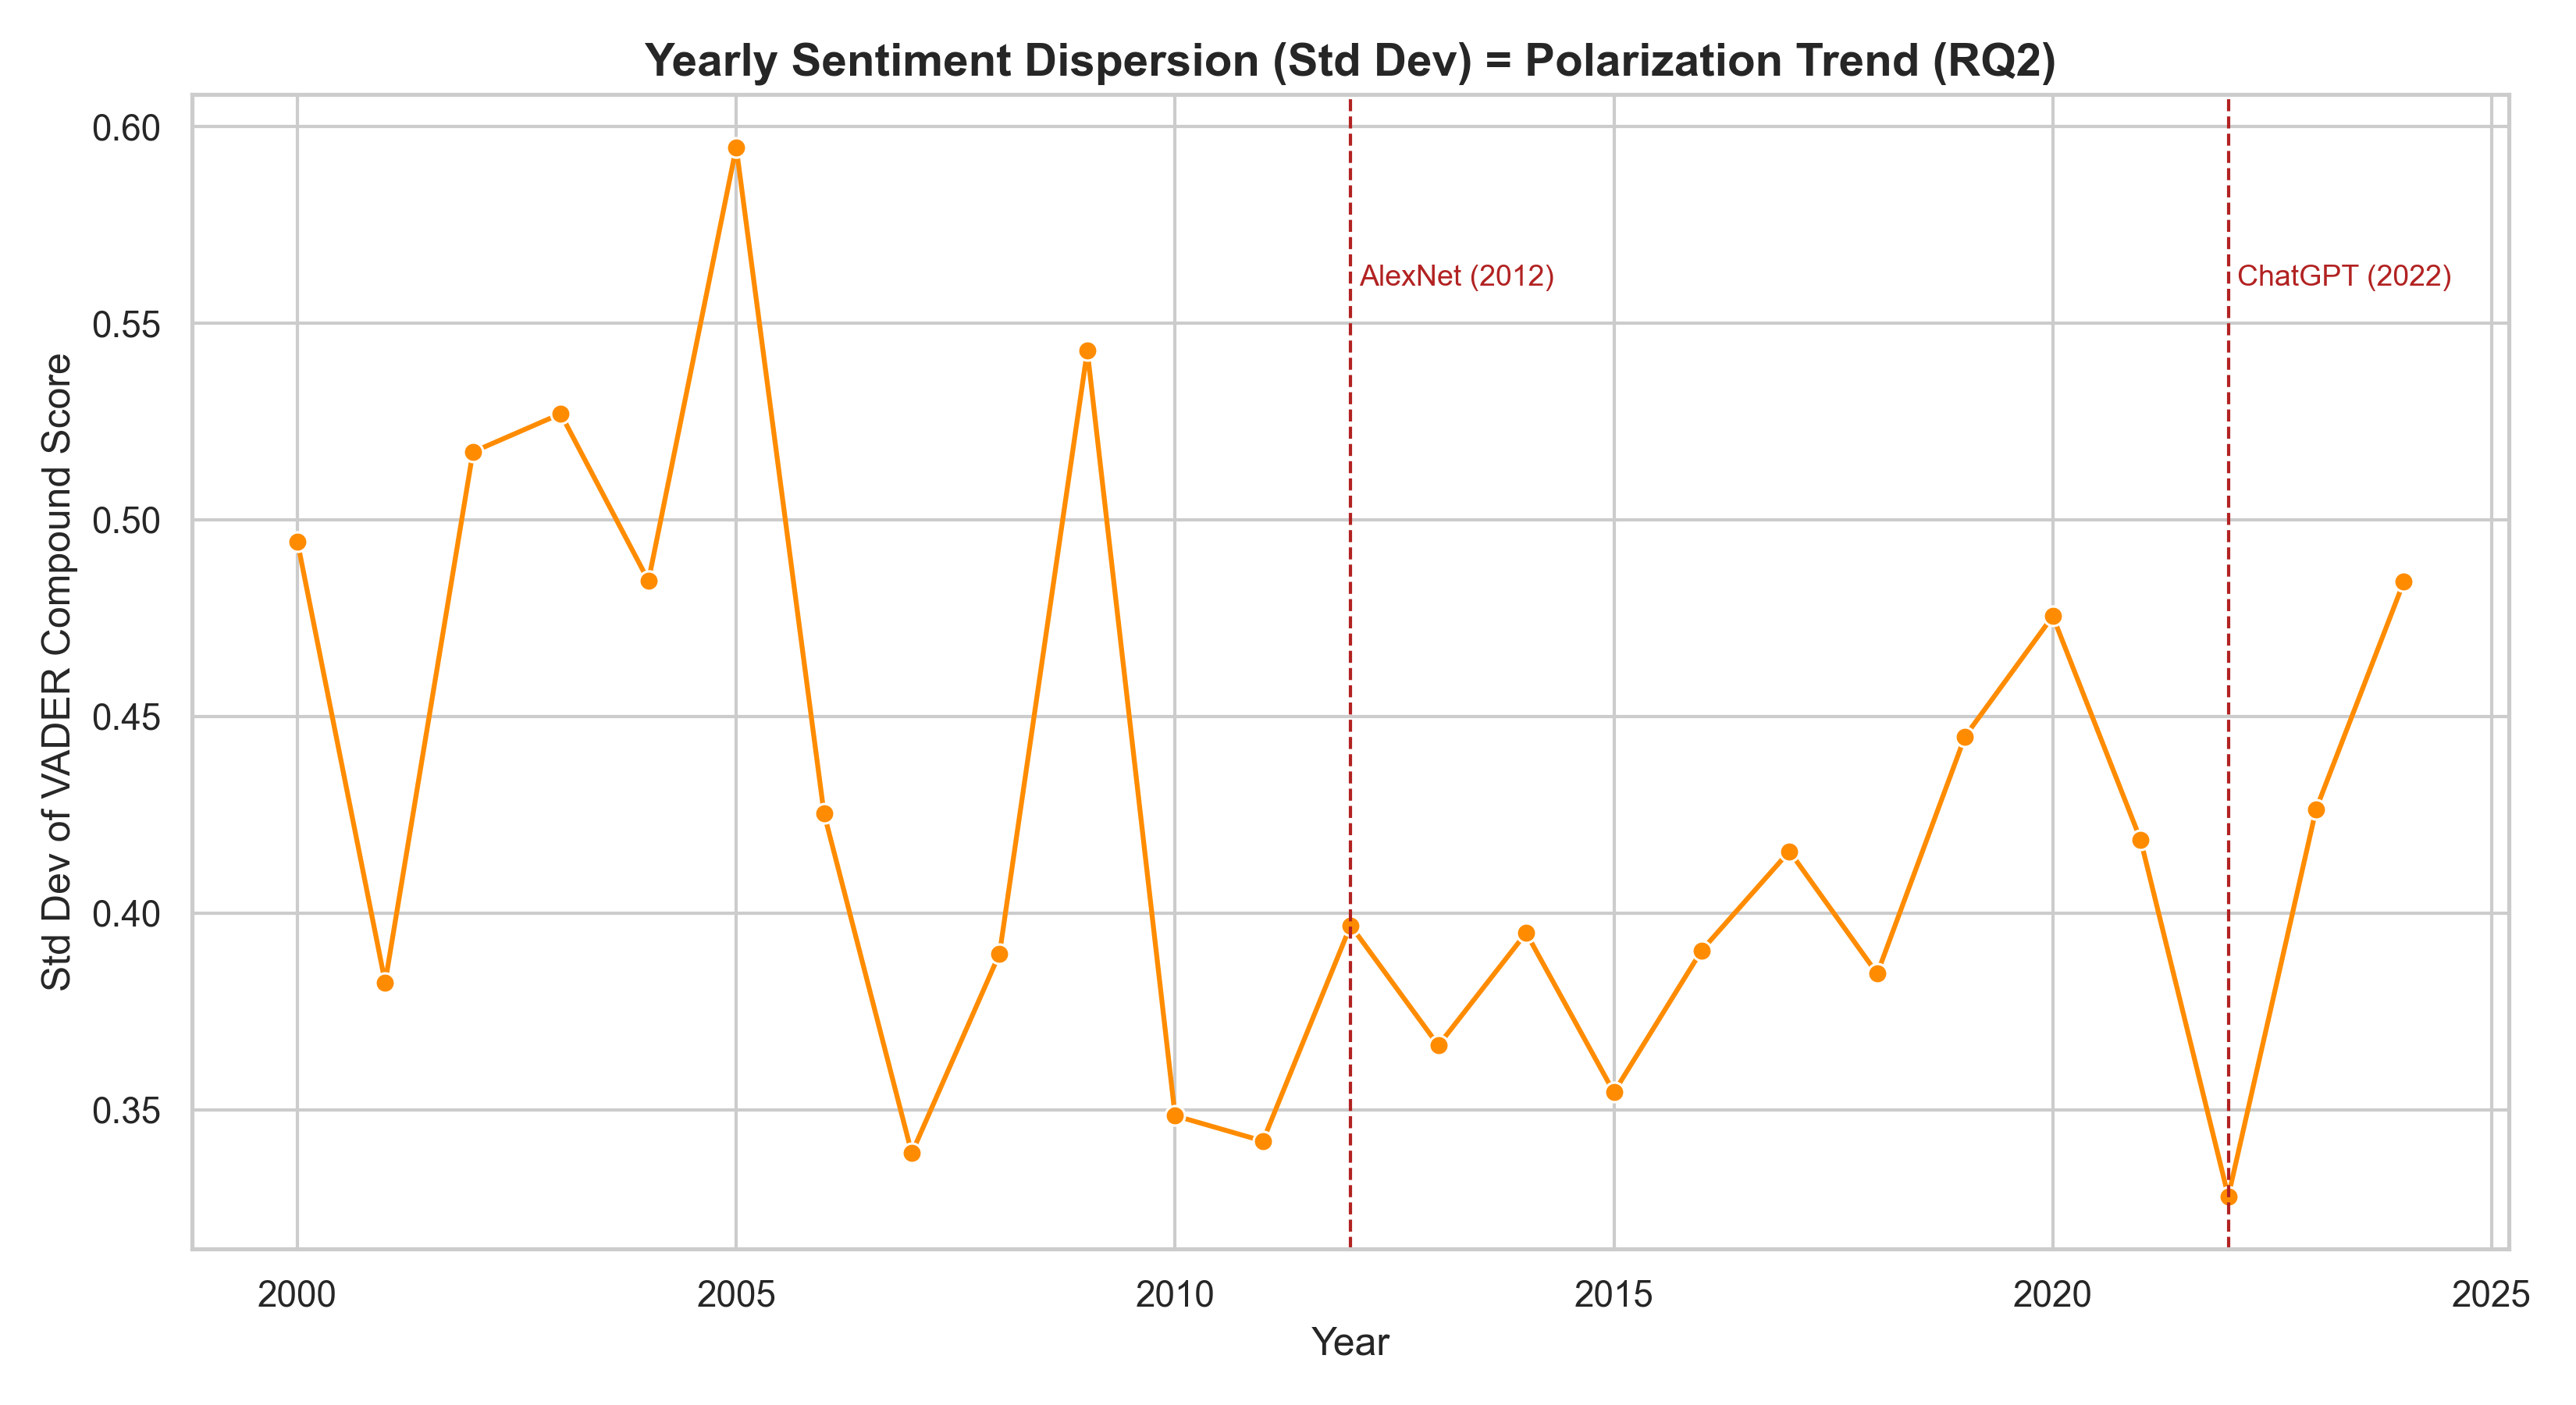
\includegraphics[width=\linewidth]{results/rq2_yearly_polarization.png}
  \caption{Annual standard deviation of abstract compound scores as a proxy
    for sentiment dispersion. Higher values indicate more polarised coverage
    within that year.}
  \label{fig:rq2-std}
\end{figure}

\begin{figure}[t]
  \centering
  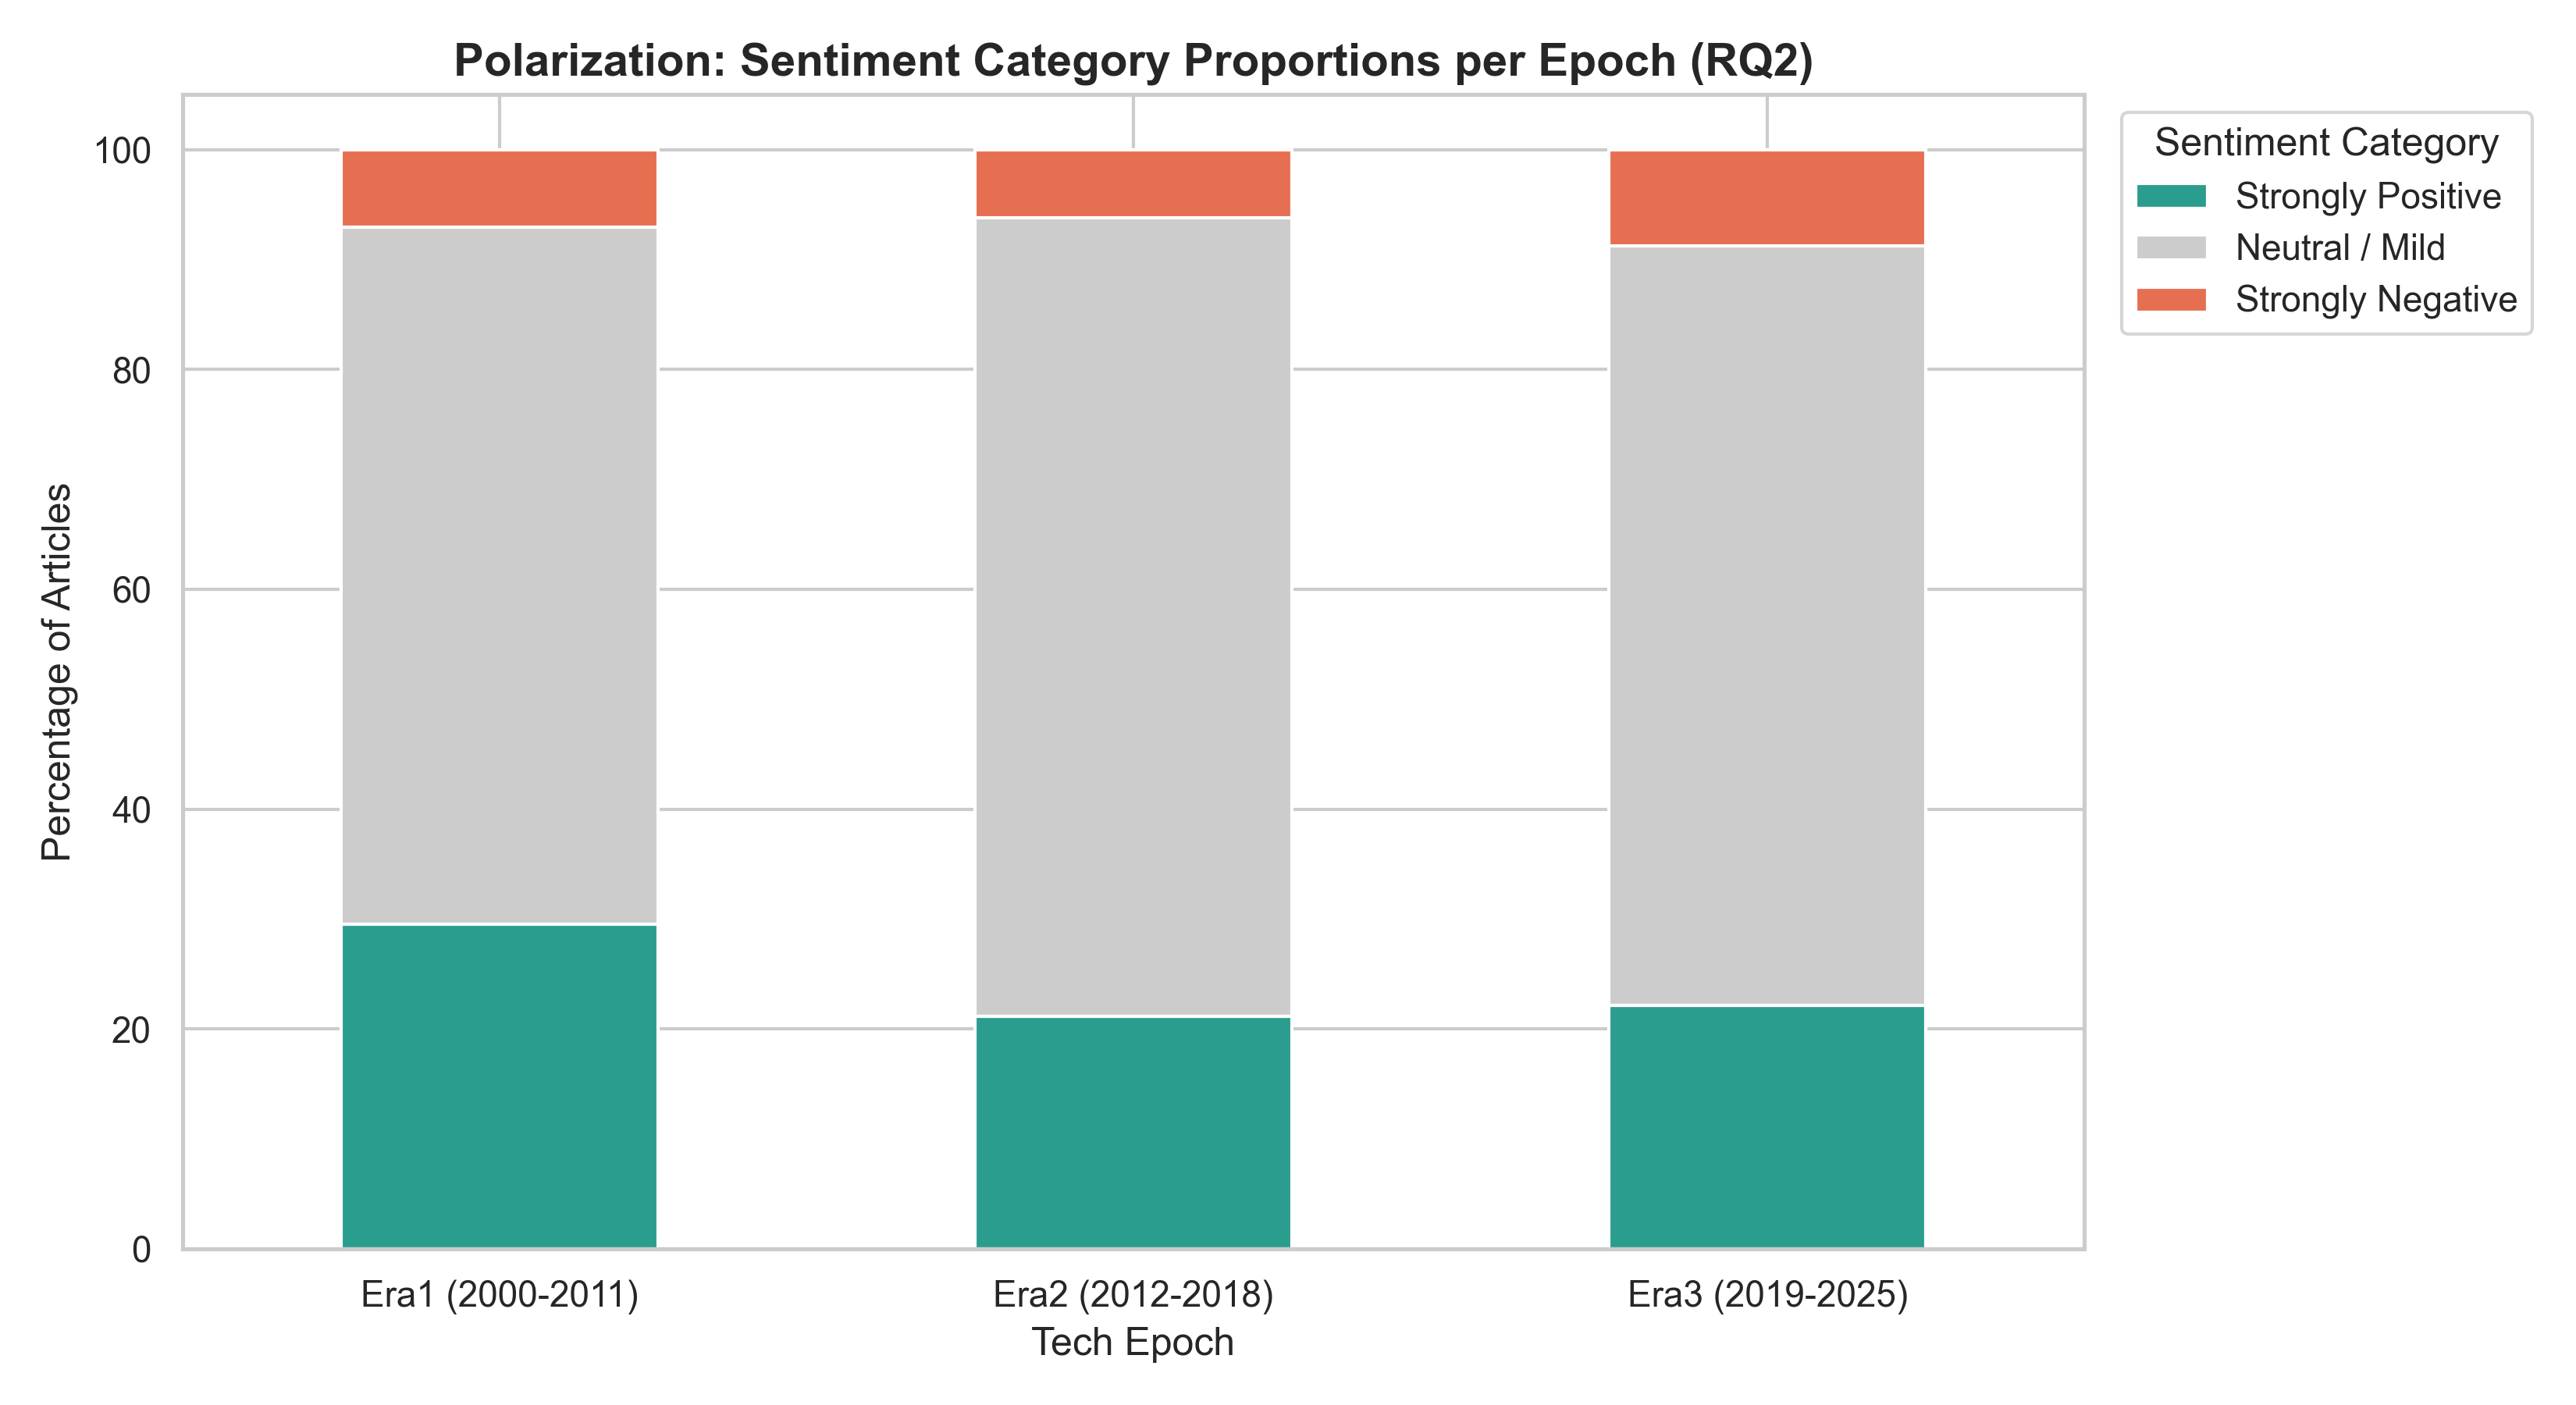
\includegraphics[width=\linewidth]{results/rq2_sentiment_proportions.png}
  \caption{Stacked bar chart showing the proportion of strongly positive,
    neutral/mild, and strongly negative articles per epoch. Era~3 has the
    highest share of strongly negative articles and the lowest share of
    neutral articles.}
  \label{fig:rq2-proportions}
\end{figure}

\subsubsection{Summary of RQ2 Findings}

The results partially support the hypothesis that sentiment polarity drifts
across technological epochs. Mean abstract sentiment declined steadily from
Era~1 to Era~3, and the full-range comparison (Era~1 vs.\ Era~3) is
statistically significant ($p = 0.042$). However, the direct Era~2 to Era~3
transition is not significant ($p = 0.798$), and all effect sizes are small
($|r| \leq 0.090$). This means the change is gradual and continuous rather
than a sudden break after ChatGPT's release. Qualitative polarisation
indicators---higher strongly-negative percentages, lower neutral share, and
a wider IQR in Era~3---do suggest that generative-AI coverage is more
emotionally charged than earlier AI reporting, but the statistical signal
from compound scores alone is modest.
